% !TeX root = ../../thesis.tex

\section{\acs{UEFI} \acf{PI}}

\cite{pi-spec} defines an implementation of the \ac{PI} process and the \ac{UEFI} environment, as well as a scalable \ac{PI} firmware storage and interface solution, which together form the basis for the development of \ac{UEFI} firmware images.
As such the following describes the rules of play for \ac{UEFI} rootkits.

\subsection{\acs{PI} Firmware Images}
\label{sec:ueif-pi:pi:pi-firmware-images}

\cite[Vol. 3, 2]{pi-spec} defines the firmware storage design.
A Firmware Image is stored in one or more non\-/volatile physical storage devices called \acp{FD}, they are most commonly flash devices \cite[Vol. 3, 2.1]{pi-spec}.
Flash often offers the ability to restrtict read and write properties differently depending on the storage region \cite[Vol. 3, 2.1.1]{pi-spec}.
\ac{UEFI} variables may reside in a region that remains read- and writable during the whole operation of a system, whereas the code storage may only be writable during the initial \ac{PI} phases.
Firmware images might be split over multiple physical \acp{FD}, but may also be inturn be logically be split into \acp{FV}.
\acp{FV} are comparable to hard drive volumes as they also are formatted with a file system, usually the \ac{PI} \ac{FFS} format defined in \cite[Vol. 3, 2.2]{pi-spec}.
The \ac{PI} \ac{FFS} is a flat file system consisting of a single list of files without any directory structure.
Parsing the volume is done by iterating over all files one by one.
Files contain code or data in the form of sections.
Sections split a file in discrete parts with the type of a section dictating its content.
File types impose restrictions on which types of sections a file may contain or not.
The full list of file types defined in the \ac{PI} specification can be seen in \autoref{tab:file-types}.
File sections are organized in trees, with encapsulating as well as leaf sections.
Together with the file section type \code{EFI\_SECTION\_FIRMWARE\_VOLUME\_IMAGE} which contains an entire \ac{PI} \ac{FV} image, this makes up for the \ac{FFS}'s lack of a directory structure.
The full list of section types can be seen in \autoref{tab:file-section-types}.

\autoref{fig:ovmf-in-uefitool} shows a firmware image opened in \program{UEFITool}, an editor for firmware images conforming to the \ac{PI} specification \cite{uefitool}.
The cursor is on the executable section of a \acs{DXE} driver.

\begin{figure}[htb]%
    \centering%
    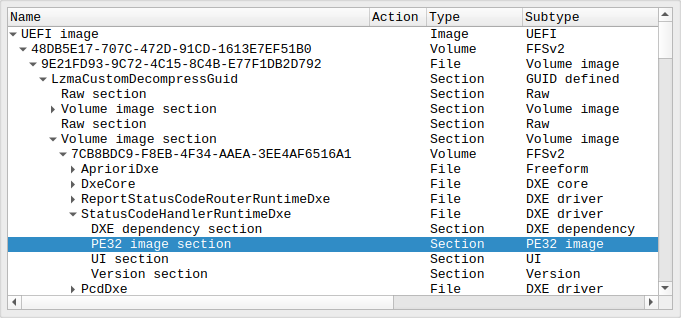
\includegraphics[width=\textwidth]{pi/ovfm_uefitool}%
    \caption{\ac{OVMF} opened in \program{UEFITool}}%
    \label{fig:ovmf-in-uefitool}%
\end{figure}


\subsection{\acs{PI} Architecture Firmware Phases}

\cite{pi-spec} defines a multi phase architecture of the \ac{PI} that can be used by system designers to implement \ac{PF}.
It is designed to be very extensible and to simplify the process of independent hardware vendors working together, when combining their software into a single \ac{PF}.
The proposed \ac{PI} architecture phases can be seen in \autoref{fig:pi-phases}, they are not entirely distinct and system designers may choose to implement phases differently.

\begin{figure}[htb]%
    \centering%
    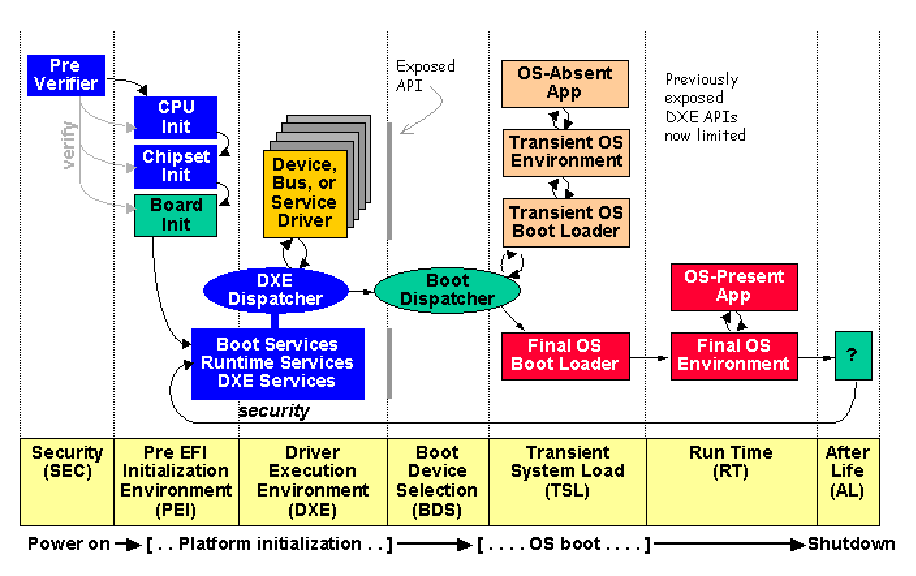
\includegraphics[width=\textwidth]{pi/pi_phases}%
    \caption{\ac{PI} Architecture Firmware Phases \cite[Figure 2-1]{pi-spec}}%
    \label{fig:pi-phases}%
\end{figure}


\subsubsection{\acf{SEC}}

The \ac{SEC} phase is the first phase performed during platform initialization.
Under its responsibilities fall handling all platform restart events, setting up temporary memory and establishing the system's root of trust.
It serves as the foundation for all secure operations on which inductive security designs rely to build a chain of trust by having a module verify the integrity of its subsequent module.
For this the \ac{SEC} phase may verify the integrity of the \ac{PEI} foundation before transfering execution to it.
As this is very specific to how the platform is implemented, the \ac{SEC} phase is only specified as the basic requirements that it needs to meet before handing over execution to the \ac{PEI} phase.
When it transfers execution, it passes information about the current state of the system, including location and size of the temporary stack, \ac{RAM}, and \ac{BFV}.
It can also optionally pass protocols for the \ac{PEI} phase to use.

\subsubsection{\acf{PEI}}

The \ac{PEI} phase configures the system to meet the minimum requirements for the \ac{DXE}.
Its job is the intialization of all system hardware requiring to be initialized beforehand, as well as the initialization of permanent memory, which is later described in \acp{HOB} to be passed off to the \ac{DXE} phase \cite[Vol. 1, 2.1]{pi-spec}.
The \ac{PEI} phase is architecturally a stripped down version of the \ac{DXE} phase, as it offers the same extensibility through modules supplied by the different \acp{OEM} responsible for the component initialization.
As the \ac{PEI}'s environment is still very restricted and the main memory only initialized towards the end of the phase, more complex processing is to be done in the \ac{DXE}.
Even though the implementation of the \ac{PEI} phase is the most hardware dependent, the core functionality of the \ac{PEI} is common to all processor architectures and offered through the \ac{PEI} foundation \cite[Vol. 1, 2.2]{pi-spec}.
It is the module initially invoked by the \ac{SEC} phase and responsible of dispatching further \acp{PEIM} and offering am intermodule communication through the management of \acp{PPI} \cite[Vol. 1, 2.5]{pi-spec}.
The \ac{PEI} foundation implements a \ac{PEI} dispatcher, who iterates over \acp{PEIM} found in \acp{FV}, to evaluate their \acp{DEPEX}.
\acp{DEPEX} are logical combinations of \acp{PPI} that must be present before loading a \ac{PEIM}.
Loading \acp{PEIM} results in the installation of new \acp{PPI} and the discovery of additional \acp{FV}.
Theis leads to previously unfullfilled \acp{DEPEX} to now be fullfilled and the dispatcher loading these \acp{PEIM} on their next evaluation.
This process is repeated until no more \acp{PEIM} are able to be dispatched.
The foundation then invokes the \emph{\ac{DXE} IPL \ac{PPI}}, which loads the \ac{DXE} foundation into memory, to then transfer execution \cite[Vol. 1, 2.6]{pi-spec}.
The \ac{BFV} containing the \ac{PEI} foundation, initially discovered by the \ac{SEC} phase, and any additionally discovered \acp{FV} are also passed off to the \ac{DXE} in the form of \acp{HOB}.

While the \ac{PEI} phase has many architecturally required \acp{PPI} that modules have to implement, the \ac{PI} also defines optional \acp{PPI}.
One of which is the \emph{Security PPI}, it used to maintain the chain of trust by offering the chance for platform builders to authenticate or log \acp{PEIM} before they are executed \cite[Vol. 1, 6.3.6]{pi-spec}.


\subsubsection{\acf{DXE}}

The \ac{DXE} phase is responsible to finalize the initialization of all platform components, as well as implementing \ac{UEFI}, the \ac{UEFI} environment and its system abstractions as they are defined in \cite{uefi-spec}.
As mentioned earlier, the \ac{DXE} phase is architecturally similar to the \ac{PEI} phase, as it also has a foundation with a dispatcher, extensibile modules in the form of \ac{DXE} drivers and uses \ac{UEFI} protocols for intermodule communication \citep[Vol. 2, 2.1]{pi-spec}.
The \ac{DXE} foundation is only dependent on the list of \acp{HOB} it receives from the previous phase, allowing it to be used with the \ac{PEI} phase or different implementations.
This also makes it possible to unload the previous stage, freeing up its memory \cite[Vol. 2, 9.1]{pi-spec}.
The \ac{DXE} foundation produces the \ac{UEFI} boot and runtime services as well as additional \ac{DXE} services and offers them through the \ac{UEFI} system table to its \ac{DXE} drivers as it can be seen in \autoref{fig:uefi-system-table}\cite[Vol. 2, 2.2.1]{pi-spec}.
\ac{DXE} drivers are very similar to \ac{UEFI} images as they even share the same entry point signature, they also come in boot and runtime variants \cite[Vol. 2, 11.2.3]{pi-spec}.
The implementation of the \ac{UEFI} system table services is done by \ac{DXE} drivers, who provide architectural protocols for the \ac{DXE} foundation to consume \cite[Vol. 2, 12.1]{pi-spec}.
Thus the foundation has to provide the most basic services, required to load and execute \ac{DXE} drivers, on its own.
\ac{DXE} drivers implementing architectural protocols are called early drivers, they can not assume that that all \ac{UEFI} system table services are already available to them and do not follow the \ac{UEFI} driver model \cite[Vol. 2, 11.2.1]{pi-spec}.
To guarantee that some of the architectural drivers are loaded before others, an \emph{a priori} file can be used.
When an \emph{a priori} file is present on a \ac{FV}, it is read to provide a deterministic order of drivers, which are to be executed before the dispatcher starts its regular \ac{DXE} driver discovery and \ac{DEPEX} evaluation on the rest of the architectural drivers \cite[Vol. 2, 10.3]{pi-spec}.
\ac{DXE} drivers which follow the \ac{UEFI} driver model have an empty \ac{DEPEX}, as installing the Driver Binding Protocol to its own image handle does not require any architectural protocols.
They are still only disptached after all architectural protocols have been installed \cite[Vol. 2, 11.2.2]{pi-spec}.
The dispatcher also makes use of a Security Architectural Protocol to authenticate each \ac{DXE} driver to deciding whether or not to execute it \cite[Vol. 2, 10.13]{pi-spec}.

When the \ac{DXE} dispatcher is unable to load any new drivers it transfers execution to the \emph{\ac{BDS} Architectural Protocol} \cite[Vol. 2, 2.4]{pi-spec}.
This presents the advancement into the \ac{BDS} phase, but not simaltaniously the end of the \ac{DXE} phase \cite[Vol. 2, 2.1]{pi-spec}.
The two phases work together until the \ac{OS} takes over control of the system with the call to \code{ExitBootServices()}.

\subsubsection{\acf{BDS}}

The \ac{BDS} phase consists of the implementation of the \emph{\ac{BDS} Architectural Protocol}.
It implements the \ac{UEFI} boot manager policy as defined in \cite[Section 3]{uefi-spec} and summarized in \autoref{sec:uefi-pi:uefi:boot-manager}.
When discovering additional \acp{FV} the \ac{DXE} dispatcher is invoked through the \ac{DXE} services.
Execution may also be returned to the \ac{DXE} phase when not enough drivers were initialized to successfully boot from a device \cite[Vol. 2, 12.2]{pi-spec}.


\subsubsection{\acf{TSL}}

The \ac{TSL} phase constist of the \ac{UEFI} \ac{OS} bootloader performing its necessary actions in preparation of assuming control over the system by calling \code{ExitBootServices()} and transfering execution to the \ac{OS} kernel \cite[Section 2.3]{tianocore-edk2-build-spec}.
The \ac{DXE} phase and all boot services are unloaded.

\subsubsection{\acf{RT}}

The \ac{RT} phase offers only minimal functionality via the remaining runtime services while the \ac{OS} owns the system \cite[Section 2.3]{tianocore-edk2-build-spec}.

\subsubsection{\acf{AL}}

The \ac{AL} phase facilitates drivers storing the system state during shutdown, sleep, hibernation and restart events \cite[Section 2.3]{tianocore-edk2-build-spec}.
